Durante la revisión del conjunto de datos ``Offendes'', se identificó que existian varias muestras que requerían reetiquetado, especialmente aquellas marcadas con lenguaje grosero. Por lo tanto, se revisó nuevamente todo el conjunto de datos, centrándose especialmente en las muestras con lenguaje grosero, y se procedió a reetiquetar manualmente teniendo en cuenta su utilidad y la percepción sobre si estos comentarios pertenecian a la categoria de groseros, ofensivos o no ofensivos en la sociedad boliviana. Este proceso se abordó detalladamente en el capítulo 4 del proyecto.

De un total de 30,416 comentarios, 2,310 pertenecían a la clase de comentarios groseros pero no ofensivos. Se reetiquetaron 142 comentarios de esta clase y posteriormente se llevó a cabo la limpieza de este conjunto de datos para su uso adecuado.

El etiquetado de los conjuntos de datos de Facebook y WhatsApp se realizó después de la limpieza de los mismos. Para esta tarea, se utilizó la técnica de aprendizaje por transferencia, que consiste en aprovechar los conocimientos adquiridos en una tarea para mejorar el rendimiento en otra tarea relacionada pero diferente. En este caso, se empleó el dataset ``Offendes'' para afinar una versión reducida del modelo BERT, el cual fue inicialmente entrenado con grandes cantidades de texto no etiquetado, como páginas web, libros y artículos de noticias.

A través de este proceso de entrenamiento masivo, el modelo aprende a comprender la estructura y el significado del lenguaje natural de manera general. Por lo tanto, cuando se adapta o afina para tareas específicas, como la clasificación de comentarios ofensivos, el modelo ya posee un conocimiento previo considerable del lenguaje, lo que permite mejorar su rendimiento en la tarea objetivo. Esto permitió que una muestra de aproximadamente 30,000 comentarios previamente etiquetados fuera utilizada para etiquetar los más de 78,000 comentarios recopilados de las redes sociales.

\textbf{BERT}

BERT, que significa Bidirectional Encoder Representations from Transformers, es un modelo de lenguaje pre entrenado desarrollado por Google, tiene una arquitectura compuesta por múltiples capas de transformers, que son unidades básicas que procesan secuencias de entrada de manera bidireccional. Esto significa que el modelo puede capturar el contexto de una palabra en una oración teniendo en cuenta tanto las palabras que la preceden como las que la siguen, lo que lo hace extremadamente efectivo para una amplia gama de tareas de procesamiento del lenguaje natural. Esto se logra mediante el entrenamiento del modelo en dos tareas: 

1.- El modelado de lenguaje enmascarado (Masked Language Modeling, MLM) que ocurre durante el entrenamiento, donde BERT recibe una secuencia de palabras de entrada y algunas de estas palabras son enmascaradas aleatoriamente. La tarea del modelo es predecir qué palabra falta en cada lugar enmascarado, lo que obliga al modelo a comprender el contexto de las palabras en una oración para poder predecir la palabra enmascarada con precisión. Ver figura \ref{fig:nlp8}

2.- Predicción de la siguiente oración: Además del MLM, BERT también se entrena en una tarea de predicción de la siguiente oración. Se le proporcionan dos oraciones y el modelo debe predecir si la segunda oración sigue a la primera en un contexto coherente o no.

\begin{figure}
	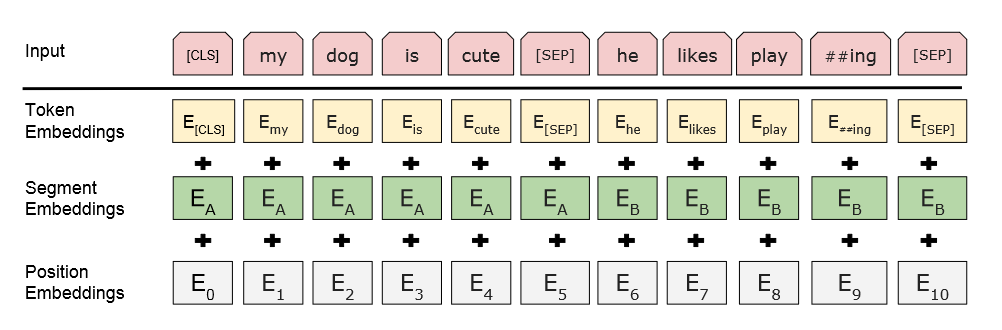
\includegraphics[width=0.65\textwidth]{capitulo3/figuras/nlp8.png}
	\caption{Representacion de entradas en BERT.}
	\floatfoot{Fuente: Pre-training of Deep Bidirectional Transformers for
		Language Understanding \cite[p. 5]{devlin2018bert} }
	\label{fig:nlp8}
\end{figure}

 \textbf{Resultados del etiquetado con Bert}

Inicialmente, se utilizó el conjunto de datos ``Offendes'' para entrenar y afinar  el modelo BERT seleccionado, con el fin de etiquetar posteriormente el conjunto de datos recolectado de la región de los valles, centrándose específicamente en el departamento de Cochabamba. Los resultados del entrenamiento de BERT con ``Offendes'' se pueden apreciar en la Tabla \ref{tbl:bert}, donde en cantidad de muestras se detalla la cantidad de comentarios usados para el conjunto de entrenamiento, validación y prueba, en precisión la exactitud del modelo en su respectivo conjunto y en error las etiquetas que se marcaron incorrectamente en cada conjunto.

\begin{table}[!ht]
	\centering
	\begin{tabular}{|c|c|c|c|}
		\hline
		\textbf{Conjunto} & \textbf{Cantidad de muestras} & \textbf{Precisión} & \textbf{Error} \\ \hline
		Entrenamiento & 21169 & 0.9297 & 0.1969 \\ 
		Validación & 4536 & 0.8715 & 0.4100 \\ 
		Prueba & 4536 & 0.8748 & 0.3932 \\ \hline
		\textbf{Total} & 30241 & - & - \\ \hline
	\end{tabular}
	\caption{Resultados del entrenamiento de Bert con Offendes}
	\label{tbl:bert}
\end{table}


Bajo el resultado obtenido descrito en la Tabla \ref{tbl:bert}, se etiquetó el conjunto de datos de Cochabamba, cuyos resultados se detallan en la Tabla \ref{tbl:cochabamba}, donde la precisión es el resultado de la revisión manual realizada después del etiquetado. Finalmente despues de todo este proceso se etiquetaron los tres últimos conjuntos de datos restantes. En la tabla \ref{tbl:santacruz} se pueden observar los resultados del etiquetado del conjunto de datos de Santa Cruz, en la tabla \ref{tbl:lapaz} se presentan los resultados obtenidos para el conjunto de datos de La Paz, y finalmente, en la tabla \ref{tbl:whatsapp} se muestran los resultados obtenidos para el conjunto de datos de WhatsApp.


\begin{table}[!ht]
	\centering
	\begin{tabular}{|c|c|c|c|}
		\hline
		\textbf{Categorías} & \textbf{Cantidad} & \textbf{No de etiquetas cambiadas} & \textbf{Precisión (\%)} \\ \hline
		Ofensivos & 8199 & 3426 & 58.22 \\ 
		No ofensivos & 26856 & 1509 & 94.38 \\ 
		Groseros & 808 & 355 & 56.06 \\ \hline
		\textbf{Total} & 35863 & 5290 & \textbf{85.25} \\ \hline
	\end{tabular}
	\caption{Resultados del etiquetado de Bert para Cochabamba}
	\label{tbl:cochabamba}
\end{table}

\begin{table}[!ht]
	\centering
	\begin{tabular}{|c|c|c|}
		\hline
		\textbf{Categoría} & \textbf{Cantidad} & \textbf{Porcentaje (\%)} \\ \hline
		Ofensivo & 3171 & 22.33 \\ 
		No ofensivo & 10650 & 75.00 \\ 
		Grosero & 379 & 2.67 \\ \hline
		\textbf{Total} & 14200 & \textbf{100.00} \\ \hline
	\end{tabular}
	\caption{Resultados del etiquetado de Bert para Santa Cruz}
	\label{tbl:santacruz}
\end{table}


\begin{table}[!ht]
	\centering
	\begin{tabular}{|c|c|c|}
		\hline
		\textbf{Categoría} & \textbf{Cantidad} & \textbf{Porcentaje (\%)} \\ \hline
		Ofensivo & 4133 & 29.62 \\ 
		No ofensivo & 9379 & 67.18 \\ 
		Grosero & 449 & 3.21 \\ \hline
		\textbf{Total} & 13961 & \textbf{100.00} \\ \hline
	\end{tabular}
	\caption{Resultados del etiquetado de Bert para La Paz}
	\label{tbl:lapaz}
\end{table}

\begin{table}[!ht]
	\centering
	\begin{tabular}{|c|c|c|}
		\hline
		\textbf{Categoría} & \textbf{Cantidad} & \textbf{Porcentaje (\%)} \\ \hline
		Ofensivo & 2050 & 14.79 \\ 
		No ofensivo & 11129 & 80.31 \\ 
		Grosero & 680 & 4.90 \\ \hline
		\textbf{Total} & 13859 & \textbf{100.00} \\ \hline
	\end{tabular}
	\caption{Resultados del etiquetado de Bert para WhatsApp}
	\label{tbl:whatsapp}
\end{table}


